\chapter{A Background on \KECCAK{}}
\label{chap:design-impl}

In this chapter we discuss details of the construction of \KECCAK{} and its standardization \SHA-$3$.

\section{\Keccak{} Description and Notations}
\Keccak{} is a family of sponge hash functions with arbitrary output length. A sponge construction consists of a permutation function, denoted by $f$, a parameter ``rate'', denoted by $r$, and a padding rule pad. The construction produces a sponge function that takes as input a bit string $N$ and output length $d$. 
It is described below.

\begin{figure}
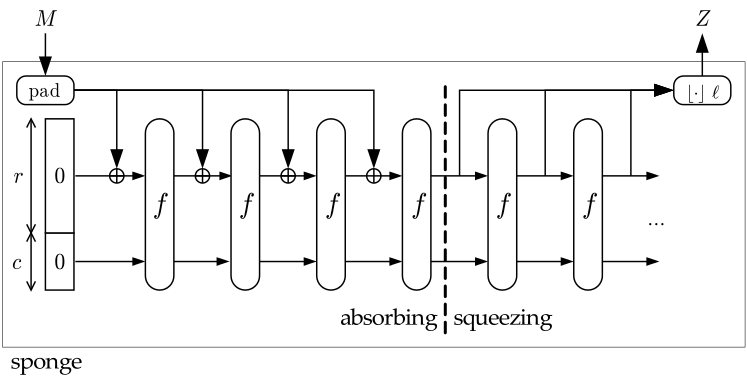
\includegraphics[width=\textwidth]{sponge.png}
\caption{The sponge construction~\cite{bertoni2011cryptographic}\label{sponge}}
\end{figure}

The input bit string $N$ is first padded based on the padding rule given by pad such that after padding, $N$ is a multiple of $r$. The padded string is then divided into blocks of length $r$, where $r$ is the rate of \KECCAK{}. The permutation function $f$ maps a string of length $b$ to another string of the same length. It operates on the $b$-bit string where the first part contains the $r$ bits of the state and the second part contains the remaining $c$ bits of the state, where $c$ is the capacity of \KECCAK{}. 

$c$ denotes the capacity which is a positive integer such that $r + c = b$. The initial state is a $b$-bit string that is set to all zeros. After the string $N$ is padded, it undergoes two phases of sponge, namely absorbing and squeezing. 

In the absorbing phase, the padded string $N^\prime$ is split into $r$-bit blocks, say $N_1, N_2, N_3,\ldots,N_m$. The first $r$ bits of the initial state is XOR-ed with the first block $N_1$ and the remaining $c$ bits are appended to the output of XOR. The XOR-ed state is fed as input to the function $f$ as shown in the diagram given in the Figure~\ref{sponge}. The output of $f$ becomes the initial state for the next block and this process repeats for all blocks of the message. After all the blocks are absorbed, the absorption phase is finished. Let the resulting state after absorption is $P$. 

In the squeezing phase, a string $Z$ is initialized with the first $r$ bits of the state $P$. The function $f$ is applied on the state $P$ and the first $r$ bits of the output state, say $P^\prime$, is appended to $Z$. The state $P^\prime$ is again passed to $f$ and this process is repeated until $|Z| \geq d$. The output of sponge construction is given by the first $d$ bits of $Z$.

The \Keccak{} family of hash functions is based on the sponge construction. The function $f$, in the sponge construction, is denoted by \Keccak-$f\left[b\right]$, where $b$ is the length of input string. Internally \Keccak-$f\left[b\right]$ consists of a round function $p$ which is recursively applied a specified number of times, say $n_r$. More precisely \Keccak-$f\left[b\right]$ function is specialization of \Keccak-$p\left[b,\,n_r\right]$ family where $n_r = 12 + 2\,l$ and $l = \log_2 (b/25)$.

The \KECCAK-$p$ permutation is defined with two parameters :
\begin{enumerate}
    \item The width of the permutation, $b$
    \item Number of rounds, $n_r$. The internal round function $rnd$ is called $n_r$ number of times.
\end{enumerate}

So,
\[
    \Keccak\text{-}f\left[b\right] = \Keccak\text{-}p\left[b,  12 + 2l\right].
\]

The state \KECCAK-$f$[$b$] consists of $b$ bits, the state is divided into slices. Here, the size of each slice is always fixed i.e. 25 bits and the number of slices depends on size $b$ bits. For \KECCAK-$f$[$1600$] state consists of $1600$ bits, where each slice contains $25$ bits and there are $1600/25 = 64$ slices. A bit position in state \KECCAK-$f$[$1600$] is determined by $x, y, $ and $z$ coordinates. $z$ coordinate determines the slice number i.e. $0 \leq z \leq 63$ for $b = 1600$ and $x, y$ determines the position of the bit in that particular slice $z$.

The round function $p$ in \Keccak{} comprises of $5$ steps, in each of which the state undergoes transformations specified by the step mapping. These step mappings are called $\theta, \rho, \pi, \chi$ and  $\iota$. These transformations are applied in sequence. A state $S$, which is a $b$-bit string, in \Keccak{} is usually denoted by a $3$-dimensional grid of size $(5 \times 5 \times w)$ as shown in the Figure~\ref{ss}. The value of $w$ depends on the parameters of \Keccak{}. For example in the case of \Keccak-$f\left[1600\right]$, $w$ is equal to $64$. It is usual practice to represent a state in terms of rows, columns, lanes, planes, sheets, slices and width of the $3$-dimensional grid.

Given a bit location $(x,y,z)$ in the grid, the corresponding row is given by $\left( S[x+i \pmod 5,y,z] : \, i \in [0,4] \right)$. Similarly the corresponding column is given by the bits $\left( S[x,y+i \pmod 5,z] : \, i \in [0,4] \right)$ and the corresponding lane is given by $\left( S[x,y,z+i \pmod w] : \, i \in [0,w-1] \right)$. 

Further, the plane corresponding to a location $(x,y,z)$, consists of 

$\left( S[x+j \pmod 5,y \pmod 5,z + i] : \, i,\,j \in [0,4] \right)$, similarly the sheets consists of $\left( S[x \pmod 5,y+j \pmod 5,z + i] : \, i,\,j \in [0,4] \right)$, and slice consists of 

$\left( S[x+j \pmod 5,y+i \pmod 5,z] : \, i,\,j \in [0,4] \right)$ bits.

Some of the above are pictorially shown in the Figure~\ref{ss}.
\begin{figure}
  \begin{tikzpicture}[on grid,scale=0.7]
  \shade[yslant=-0.5,right color=gray!10, left color=black!40] (0,2) rectangle +(5,1) node[xshift=-1.2cm, yshift=0.2cm] at (0,2){ a row($5$-bits)};
%lane 1x1
  \shade[yslant=-0.5,left color=black!40,  color=black!10] (4,4) rectangle +(1,1);
%column
  \draw[yslant=-0.5,pattern=north east hatch,  pattern color=black!70, hatch distance=3pt, hatch thickness=0.5pt] (2,0) rectangle +(1,5)
  node[xshift=-0.8cm, yshift=-0.2cm] at (2,0){ a column($5$-bits)};
  
  \draw[yslant=-0.5, dashed] (0,0) grid (5,5);
  \shade[yslant=0.5,right color=black!60,left color=black!40](5,-1) rectangle +(8,1);
  \draw[yslant=0.5] (5,-5) grid (13,0);
  \node at (15.9,6.5){a lane($w$-bits)};
%slice front
  \draw[yslant=0.5,pattern=north east hatch,  pattern color=black!70, hatch distance=3pt, hatch thickness=0.5pt](7,-5) rectangle +(1,5)
   node[xshift=1.5cm, yshift=-0.1cm] at (7,-5){ a slice($5\times 5$-bits)};
%row front
 \shade[yslant=0.5,left color=black!20,right color=black!70] (5,-3) rectangle +(1,1);
%top shade
  \shade[yslant=0.5,xslant=-1,bottom color=gray!5,top color=gray!60] (5,0) rectangle +(8,5);
  \shade[yslant=0.5,xslant=-1, bottom color=black!40,top color=black!60](5,0) 
  rectangle +(8,1); 
 %slice top 
  \draw[yslant=0.5,xslant=-1,pattern=north east hatch,  pattern color=black, hatch distance=3pt, hatch thickness=0.5pt] (7,0) rectangle +(1,5);
%column top
  \draw[yslant=0.5,xslant=-1,pattern=north east hatch,  pattern color=black, hatch distance=3pt, hatch thickness=0.5pt] (5,2) rectangle +(1,1);
  
  \draw[yslant=0.5,xslant=-1] (5,0) grid (13,5);
  \end{tikzpicture}
\caption{The \KECCAK{} State \label{ss}}
\end{figure}
%

\section{\textsc{\Keccak-$p$ Permutation}}
$\Rnd$\;- A round of \KECCAK-$p$ permutation, it consists of five transformations: {$\theta,\rho,\pi,\chi,\iota$}. 
In the following, we provide a brief description of the step mappings.
 Let $A$ and $B$ respectively denote input and output states of a step mapping.
\begin{enumerate}
    \item $\theta$ ({\bf theta}): The theta step XORs each bit in the state with the parities of two neighboring columns. 
        Parity of a column is defined as the $XOR$ of all the bits present in that column, i.e. $\oplus_{y = 0}^{4} A[x, y, z]$. For a given bit position $(x, y, z)$, one column is $((x - 1) \bmod 5, z) $ and the other is $((x+1)\bmod 5, (z - 1) \bmod w)$.
    
    Thus, if we have $A$ as the input state to $\theta$ then the output state $B$ is :
    \begin{align}\nonumber
        B\left[x, y, z\right] &= A\left[x, y, z\right] \oplus P\left[ (x - 1) \bmod 5 ,\, z \right] \\
        &\hspace{1.3cm}\oplus P\left[ (x + 1) \bmod 5 ,\, (z - 1) \bmod w \right]
    \end{align}
    where $P[x, z]$ represents the parity of the column represented by $(x, z)$ and 
    \[
        P[x, z]  = \oplus_{y = 0}^{4} A[x, y, z]
    \]
    $\theta$ is a linear transformation, therefore it doesn't introduce any non-linear terms if the state is linear.
    %%% CHECK: Done
    \vskip5pt
    \item $\rho$ ({\bf rho}): This step rotates each lane by a constant value towards the MSB i.e., 
    \begin{align}
        B[x, \,y,\, z] = A[x, \,y, \,z + \rho(x, y) \bmod w ],
    \end{align}
    where $\rho(x, y)$ is the constant for lane $(x, y)$. 
    
        The constant value $\rho(x, y)$ is specified for each lane in the construction of \Keccak{} as shown in Table : ~\ref{tab4} 
        
        \begin{table}[h!]
            \begin{center}
                \begin{tabular}{c|c|c|c|c|c}
                    \textbf{.} & \textbf{x = 3} & \textbf{x = 4} & \textbf{x = 0} & \textbf{x = 1} & \textbf{x = 2}\\ % <-- added & and content for each column
                    \hline
                    \textbf{y = 2} & 153 & 231 & 3 & 10 & 171\\ % <--
                    \hline
                    \textbf{y = 1} & 55 & 276 & 36 & 300 & 6\\ % <--
                    \hline
                    \textbf{y = 0} & 28 & 91 & 0 & 1 & 190\\ % <--
                    \hline
                    \textbf{y = 0} & 120 & 78 & 210 & 66 & 253\\ % <--
                    \hline
                    \textbf{y = 4} & 21 & 136 & 105 & 45 & 15\\ % <--
                    \hline
                \end{tabular}
                \caption{Values of $\rho$ constants for all lanes}\label{tab4}
            \end{center}
        \end{table}                                                                 
        $\rho$ is also a linear step mapping.

    \vskip5pt
    \item $\pi$ ({\bf pi}): It permutes the positions of lanes. The new position of a lane is determined by a matrix, 
    \begin{align}
    \begin{bmatrix} x'\\ y'\end{bmatrix} = 
    \begin{bmatrix} 0 & 1 \\ 2 &  3 \end{bmatrix} \cdot \begin{bmatrix} x\\ y\end{bmatrix},
    \end{align}
    where $(x', y')$ is the position of lane $(x, y)$ after $\pi$ step.
        $\pi$ is also a linear step mapping.
    \vskip5pt
    \item $\chi$ ({\bf chi}): In this operation each bit in the original state is XOR-ed with a non-linear function of next two bits in the same row i.e.,
    \begin{align}\nonumber
        B[x, y, z] &=  A[x, y, z] \;\oplus \\
        & \hspace{0.5cm} \left( \left(A[ (x + 1 )\bmod 5, y, z] \oplus 1\right) \cdot  A[ (x + 2) \bmod 5, y, z] ) \right).
    \end{align}
    
    $\chi$ is the only non-linear operation among the $5$ step mappings in \KECCAK{}.
    
    \vskip5pt
    \item $\iota$ ({\bf iota}): This step mapping only modifies the $(0, 0)$ lane depending on the round number i.e., 
    \begin{align}
       B[0, 0] = A[0, 0] \oplus RC_i,
   \end{align}
    where $RC_i$ is round constant that depends on the round number. The remaining $24$ lanes remain unaffected.
    
    All the rounds are identical but the symmetry is destroyed by the step $\iota$ by the addition of a round constant to a particular lane, where the round constant is dependent on the round index.
    All the additions and multiplications in the operations defined above are in $\textbf{GF}(2)$.
\end{enumerate}
Thus a round in \Keccak{} is given by ${\tt Round}(A, i_r) = \iota( \chi( \pi ( \rho ( \theta ( A ) ) ) ) , i_r)$, where $A$ is the state and $i_r$ is the round index. In the \Keccak-$p[b, n_r]$, $n_r$ iterations of ${\tt Round}(\cdot)$ is applied on the state $A$.

%% Check
The \SHA-3 hash function is \Keccak-$p[b, 12 + 2\,l]$, where $w = b/25$ and $l = \log_{2}(w)$. The value of $b$ is $1600$, so we have $l = 6$. Thus the $f$ function in \SHA-3 is \Keccak-$p[1600, 24]$.

The \Keccak{} team denotes the instances of \Keccak{} by $\Keccak[r,c]$, where $r=1600-c$ and the capacity $c$ is chosen to be twice the size of hash output $d$, to avoid generic attacks with expected cost below $2^d$. Thus the hash function with output length $d$ is denoted by 
\begin{eqnarray}
\mbox{\Keccak-$d$}  &=& \Keccak[r:=1600-2d,\;c:=2d],
\end{eqnarray}
\begin{table}
\begin{center}
\caption{Parameters and Symbols used in \KECCAK{}}\label{tab3}
\begin{tabular}{|c|l|}
\hline
Symbol & Description\\
\hline
$b$ & The width of \KECCAK{} state in bits \\
$r$ & rate of a sponge function \\
$c$ & capacity of a sponge function\\
$d$ & Length of the hash of a hash function\\
$f$ & The function used for sponge construction \\
$i_r$ & Round index for a \KECCAK-$p$ permutation\\
$n_r$ & Number of rounds for \KECCAK-$p$ permutation\\
pad & padding rule for the sponge construction\\
$w$ & Number of bits in a lane in \KECCAK{} state\\
$\theta,\rho,\pi,\chi,\iota$ & A round is comprised of these five step mappings \\
SPONGE$[f, $pad$, r]$ & Sponge function in which the underlying permutation function is $f$,\\ & padding rule is pad and rate is $r$ \\
\hline
\end{tabular}
\end{center}
\end{table}

Table~\ref{tab3} shows various parameters and other variables related to \KECCAK{}

\section{Sponge Construction}

The sponge construction is an iterated construction for building a function SPONGE$[f, $pad$, r]$ with arbitrary input and output lengths which is built on three components : fixed length permutation function $f$ which operates on a state of fixed length $b$, pad - a padding rule and $r$ - a parameter called rate.

The function produced from this construction is known as the sponge function which is denoted by SPONGE$[f, $pad$, r](N, d)$. It takes as input $N$ and $d$ where $N$ is the input bit string of any length and $d$ is the length of the output string.

\section{\KECCAK{} Specification}

\KECCAK{} is a family of sponge functions, the padding rule for \KECCAK{} is called multi-rate padding specified in section~\ref{padding}. \SHA-3 functions are defined by \KECCAK{}[$c$] which is a further smaller family of \KECCAK{} functions specified in section~\ref{keccakc}.

\subsection{Padding Rule Specification}
\label{padding}

The padding rule followed by \KECCAK{} is \textbf{pad10*1}. The asterisk in the padding rule indicates that $0$ bit is either not present or is repeated as required so that the length of output string after padding is a multiple of the block length (i.e. $r$). So, the padding rule is that the input string is appended with a $1$ bit followed by some number of $0$ bits and followed by $1$ bit.

\subsection{\KECCAK{}$[c]$ Specification}
\label{keccakc}

\KECCAK{} is a family of sponge functions with the \KECCAK{}-$p[b, 12 + 2l]$ permutation function, \textbf{pad10*1} as the padding rule and rate $r$, such that $r + c = b$. The family of sponge functions is parameterized for any width $b$ in $[25, 50,100,200,400,800,1600]$ with any rate $r$ and capacity $c$ such that $r + c = b$.

When $b = 1600$, the \KECCAK{} family is denoted by \KECCAK{}[$c$], where $c$ is the capacity, so the rate depends on the value of the $c$. So, 
\[\KECCAK{}[c] = \text{SPONGE}[\KECCAK{}\text{-}p[1600, 24], pad10*1, 1600-c]\]
For an input $N$ bit string and digest length $d$, the specification is 
\[\KECCAK{}[c](N, d) = \text{SPONGE}[\KECCAK{}\text{-}p[1600, 24], pad10*1, 1600-c](N, d)\]
\section{SHA-3 Functions}

The \SHA-3 hash family supports minimum four different output length $d \in \{224,256,384,512\}$. In the \Keccak-384, the size of $c = 2\cdot d = 768$ and the rate $r = 1600 - c = 1600 - 768 = 832= 13\cdot 64$.

\subsection{SHA-3 Hash Functions}

There are $4$ \SHA-3 hash functions, which are defined from \KECCAK{}[$c$] specified in ~\ref{keccakc}. These functions specify the input message along with the length of the digest $d$.

\[
   \text{ \SHA3-}d\;(M) = \KECCAK{}[c]\;(M||01 , d), \text{ where } c = 2*d
\]

Since there are two types of functions for \SHA-3 i.e. hash functions and Extendable-output functions. So, in order to differentiate the inputs to $\KECCAK{}[c]$ the message is appended with a suffix $01$ i.e. $M||01$.For each of four hash functions the capacity $c = 2\cdot d$. The four hash functions are \SHA3-224, \SHA3-256, \SHA3-384 and \SHA3-512

\subsection{SHA-3 Extendable-Output Functions}

The two \SHA-3 XOFs are \textsc{Shake}128, \textsc{Shake}256 which are defined from the \KECCAK{}[$c$] function.

\[
    \text{SHAKE}128\;(M,d) = \KECCAK{}[256]\;(M||1111 , d)
\]
\[
    \text{SHAKE}256\;(M,d) = \KECCAK{}[512]\;(M||1111 , d)
\]

\section{Notations and Observations}

In the following chapters, we study the cryptanalysis of \KECCAK{} which uses certain notations and observations, in this section, we study them.
In the analysis, we will represent a state by the lanes. There are in total $5\times 5$ lanes. Each lane in a state will be represented by a variable which is a $64$-bit array. 
A variable with a number in round bracket $"( . )"$ represents the shift of the bits in array towards MSB. A variable with a number in square bracket $"[ . ]"$ represents the bit value of the variable at that index. If there are multiple numbers in the square bracket then it represents the corresponding bit values.

%% More details

We are going to use the following observations in our analysis.
\begin{enumerate}
\item \label{ob1}\textbf{Observation 1:} $\chi$ is a row-dependent operation. Guo \etal in~\cite{guo2016linear}, observed that if we know all the bits of a row then we can invert $\chi$ for that row. It is depicted in the Figure~\ref{chi_inv}.
%------------------------------------------------------
\begin{figure}
\begin{center}
\begin{tikzpicture}[ampersand replacement=\&]
\matrix (m1) [matrix of nodes,
nodes={inner sep=5pt,text width=0.5cm,align=center,minimum height=.5cm, draw,text height=1em,text depth=.2em}
]{
    $a_0$ \& $a_1$\& $a_2$ \& $a_3$ \& $a_4$\\
};

\matrix (m2) [right = 1.2cm of m1, matrix of nodes,
nodes={inner sep=5pt,text width=0.5cm,align=center,minimum height=.5cm, draw,text height=1em,text depth=.2em}
]{
    $a_0^\prime$ \& $a_1^\prime$\& $a_2^\prime$ \& $a_3^\prime$ \& $a_4^\prime$\\
};
\draw[->, very thick] (m1)-- node[above, pos=0.5] {$\chi^{-1}$} (m2);
\end{tikzpicture}
\end{center}
\caption{Computation of $\chi^{-1}$ for full row \label{chi_inv}}
\end{figure}
%------------------------------------------------------
% check it for correctness
\begin{align}
a_i^\prime = a_i \oplus \left( a_{i+1} \oplus 1\right) \cdot \left( a_{i+2} \oplus \left( a_{i+3} \oplus 1 \right) \cdot a_{i+4}\right)
\end{align}


\item \label{ob2}\textbf{Observation 2:} When only one output bit is known after $\chi$ step, then the corresponding input bits have $2^4$ possibilities. Kumar \etal\cite{kumar2018cryptanalysis} gave a way to fix the first output bit to be the same as the input bit and the second bit as $1$. It is shown in the Figure~\ref{chi_inv2}.

%------------------------------------------------------
\begin{figure}[ht]
\begin{center}
\begin{tikzpicture}[ampersand replacement=\&]
\matrix (m1) [matrix of nodes,
nodes={inner sep=5pt,text width=0.5cm,align=center,minimum height=.5cm, draw,text height=1em,text depth=.2em}
]{
    $a_0$ \& $*$ \& $*$ \& $*$ \& $*$\\
};

\matrix (m2) [right = 1.2cm of m1, matrix of nodes,
nodes={inner sep=5pt,text width=0.5cm,align=center,minimum height=.5cm, draw,text height=1em,text depth=.2em}
]{
    $a_0$ \& $1$ \& $*$ \& $*$ \& $*$\\
};
\draw[->, very thick] (m1)-- node[above, pos=0.5] {$\chi^{-1}$} (m2);
\end{tikzpicture}
\end{center}
\caption{Computation of $\chi^{-1}$ when only 1-bit is known in row \label{chi_inv2}}
\end{figure}

\item \label{ob3}\textbf{Observation 3:} Guo \etal in~\cite{guo2016linear} observed that when $4$ out of $5$ output bits are known after $\chi$ step then we can establish $4$ linear equations on the input bits of $\chi$.

$a_0, a_1, a_2, a_3, a_4$ are the output bits of $\chi$ and $a_0^\prime, a_1^\prime, a_2^\prime, a_3^\prime, a_4^\prime$ are the input bits.
\begin{align}\label{eq:a0}
a_0^\prime = a_0 \oplus \left( a_{1} \oplus 1\right) \cdot \left( a_{2} \oplus \left( a_{3} \oplus 1 \right) \cdot a_{4}\right)
\end{align}
\begin{align}\label{eq:a1}
a_1^\prime = a_1 \oplus \left( a_{2} \oplus 1\right) \cdot \left( a_{3} \oplus \left( a_{4} \oplus 1 \right) \cdot a_{0}\right)
\end{align}
\begin{align}\label{eq:a2}
a_2^\prime = a_2 \oplus \left( a_{3} \oplus 1\right) \cdot \left( a_{4} \oplus \left( a_{0} \oplus 1 \right) \cdot a_{1}\right)
\end{align}
\begin{align}\label{eq:a3}
a_3^\prime = a_3 \oplus \left( a_{4} \oplus 1\right) \cdot \left( a_{0} \oplus \left( a_{1} \oplus 1 \right) \cdot a_{2}\right)
\end{align}
\begin{align}\label{eq:a4}
a_4^\prime = a_4 \oplus \left( a_{0} \oplus 1\right) \cdot \left( a_{1} \oplus \left( a_{2} \oplus 1 \right) \cdot a_{3}\right)
\end{align}

If we know the values of $a_0, a_1, a_2, a_3$ and with the above $5$ equations in terms of the unknown output bit i.e. $a_4$. Then we can establish $4$ linear equations by eliminating $a_4$ from the above $5$ equations.

So, from equation \ref{eq:a4} we get,
\begin{align}\label{eq:a4_2}
 a_4 = a_4^\prime \oplus \left( a_{0} \oplus 1\right) \cdot \left( a_{1} \oplus \left( a_{2} \oplus 1 \right) \cdot a_{3}\right)
\end{align}

As the values of $a_0,a_1,a_2,a_3$ are known, from equation \ref{eq:a4_2} we get
\begin{align}\label{eq:a4_3}
a_4 = a_4^\prime \oplus c
\end{align}
where $c = \left( a_{0} \oplus 1\right) \cdot \left( a_{1} \oplus \left( a_{2} \oplus 1 \right) \cdot a_{3}\right) $

Substituting value of $a_4$ from equation \ref{eq:a4_3} in \ref{eq:a0}. We get, 
\begin{align}\label{eq:a0_2}
a_0^\prime = a_0 \oplus \left( a_{1} \oplus 1\right) \cdot \left( a_{2} \oplus \left( a_{3} \oplus 1 \right) \cdot \left( a_4^\prime \oplus c \right)  \right)
\end{align}
Similarly, we can substitute the values of $a_4$ in equations \ref{eq:a1}, \ref{eq:a2}, \ref{eq:a3}.

\item \label{ob4}\textbf{Observation 4:} $\chi$ is an interesting non-linear operation. If we consider:
\begin{figure}[H]
    \begin{center}
        \begin{tikzpicture}[ampersand replacement=\&]
        \matrix (m1) [matrix of nodes,
        nodes={inner sep=5pt,text width=0.5cm,align=center,minimum height=.5cm, draw,text height=1em,text depth=.2em}
        ]{
            $a_0$ \& $a_1$\& $a_2$ \& $a_3$ \& $a_4$\\
        };
        
        \matrix (m2) [right = 1.2cm of m1, matrix of nodes,
        nodes={inner sep=5pt,text width=0.5cm,align=center,minimum height=.5cm, draw,text height=1em,text depth=.2em}
        ]{
            $b_0$ \& $b_1$\& $b_2$ \& $b_3$ \& $b_4$\\
        };
        \draw[->, very thick] (m1)-- node[above, pos=0.5] {$\chi$} (m2);
        \end{tikzpicture}
    \end{center}
    \caption{Computation of $\chi$ for full row \label{chi_inv}}
\end{figure}

Then,
\begin{align}\label{eq:b0}
b_0 = a_0 \oplus \left( a_1 \oplus 1 \right) \cdot a_2
\end{align}

similarly,
\begin{align}\label{eq:b1}
b_1 = a_1 \oplus \left( a_2 \oplus 1 \right) \cdot a_3
\end{align}

By equation~\ref{eq:b1} we have
\begin{align}\label{eq:b1_2}
b_1 \cdot a_2 = \left( a_1 \oplus \left( a_2 \oplus 1 \right) \cdot a_3 \right) \cdot a_2 = a_1 \cdot a_2
\end{align}

Similarly,
\begin{align}\label{eq:b1_3}
\left(b_1 \oplus 1 \right) \cdot a_2 = \left( \left( a_1 \oplus \left( a_2 \oplus 1 \right) \cdot a_3 \right) \oplus 1 \right) \cdot a_2 = \left( a_1 \oplus 1 \right) \cdot a_2
\end{align}

Using equation~\ref{eq:b1_3} and substituting in~\ref{eq:b0}. We obtain,
\begin{align}\label{eq:b0_2}
b_0 = a_0 \oplus \left( b_1 \oplus 1 \right) \cdot a_2
\end{align}

If the value of $b_1 = 1$ then we obtain a new relation for $b_0$,
\begin{align}\label{eq:b0_3}
b_0 = a_0 \oplus \left( 1 \oplus 1 \right) \cdot a_2 = a_0 \oplus \left( 0 \right) \cdot a_2 = a_0 \oplus 0 = a_0
\end{align}

So we observe that when output bit $b_1 = 1$ then we can say that $a_0 = b_0$. This observation is useful in cases where 2 consecutive output bits i.e. $b_i, \; b_{i+1}$ of step $\chi$ are known and $b_{i+1} = 1$, then we can imply that $a_i = b_i$.

\item \label{ob5}\textbf{Observation 5:}
\begin{figure}[H]
    \centering
    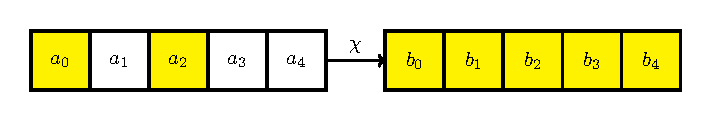
\includegraphics{chistep.pdf}
    \caption{Linear variables after $\chi$}
    \label{fig:chistep}
\end{figure}

Yellow colored bits in Figure~\ref{fig:chistep} represent linear variable and white colored bit represents constant ($0$ or $1$). This figure demonstrates the spread of linear variables after applying $\chi$. The equation for $\chi$ operation is:

\begin{align}\label{eq:chi}
b_i = a_i \oplus \left( a_{i+1} \oplus 1 \right) \cdot a_{i+2}
\end{align}

Based on equation~\ref{eq:chi}, we can say that $b_i$ is non-linear if both $a_{i+1}$ and $a_{i+2}$ are linear variables. The input row to $\chi$ step in Figure~\ref{fig:chistep} has no two adjacent bits as linear variables due to which there are no non-linear terms in the output row.

%------------------------------------------------------
\end{enumerate}
